\subsection{L'interface Utilisateur}

\begin{frame}{Nos réalisations}{Interface Utilisateur}
    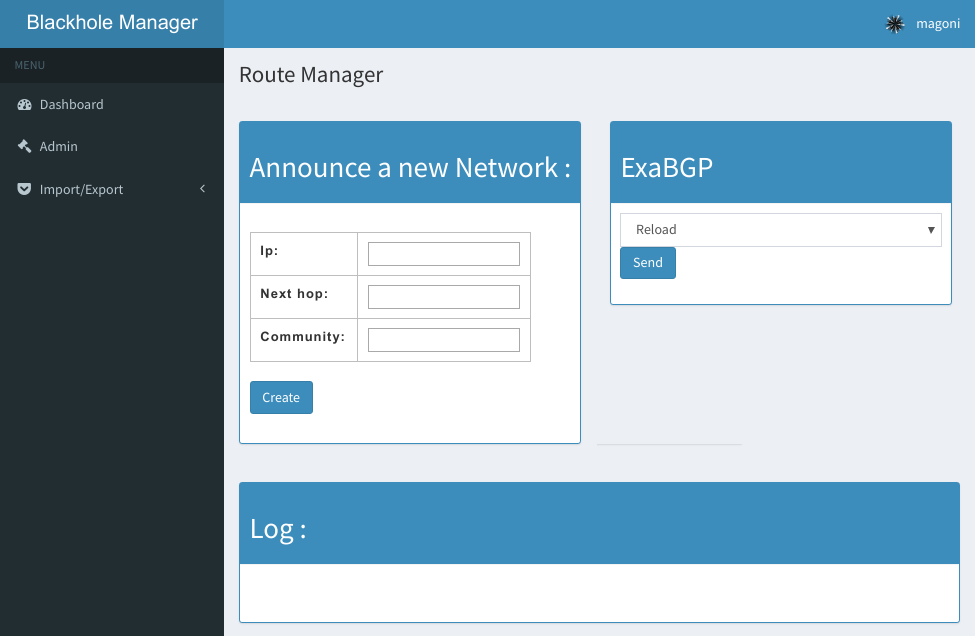
\includegraphics[width=\textwidth]{ui_upper.png}
\end{frame}

\begin{frame}{Nos réalisations}{Interface Utilisateur}
    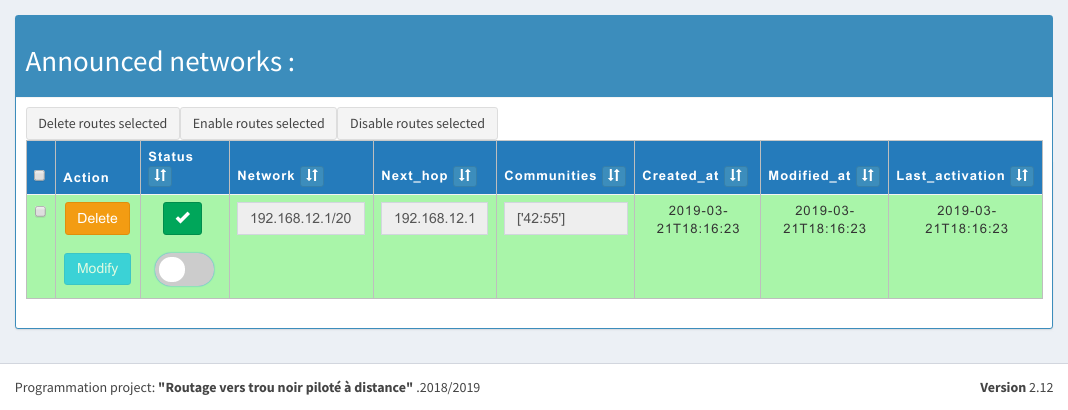
\includegraphics[width=\textwidth]{ui_lower.png}
\end{frame}

\begin{frame}{Nos réalisations}{Fonctionnement}
    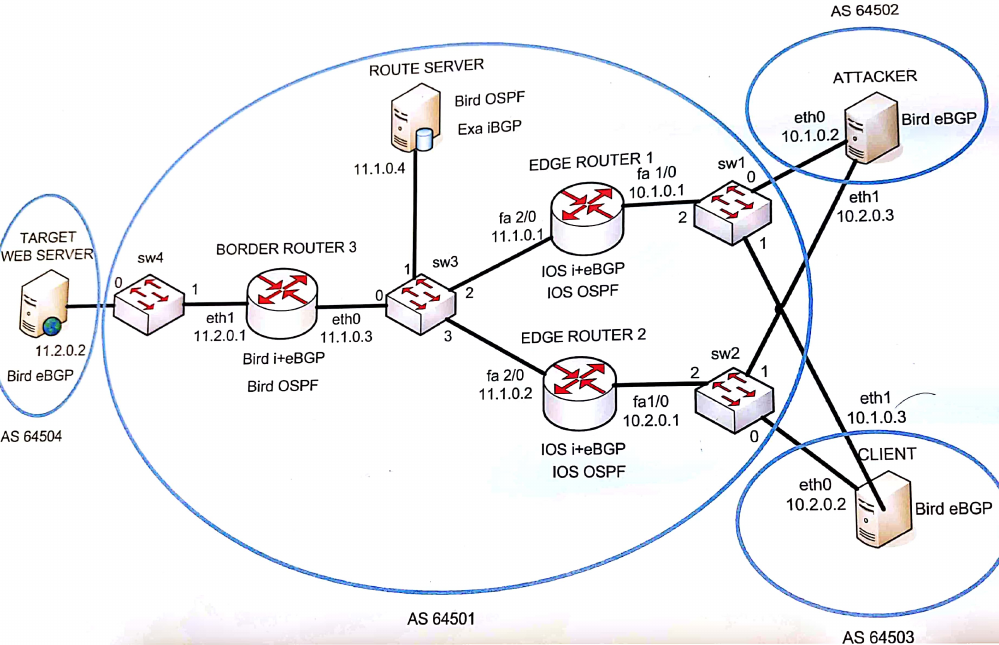
\includegraphics[width=\textwidth]{topologie.png}
\end{frame}

\begin{frame}{Nos réalisations}{Redirection vers trou noir par la destination}
    {\large \centerline{État avant la redirection}}
    \begin{minipage}{0.49\textwidth}
        \begin{figure}[H]
            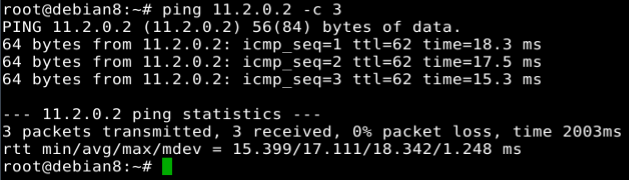
\includegraphics[width=\textwidth]{client_before_ban_v2.png}
            \caption*{Client}
        \end{figure}
    \end{minipage}
    \hfill
    \begin{minipage}{0.49\textwidth}
        \begin{figure}[H]
            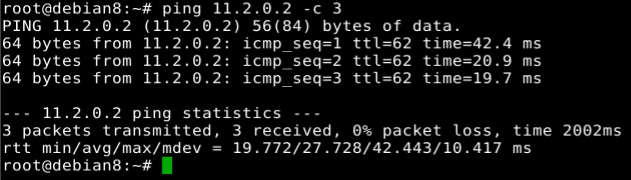
\includegraphics[width=\textwidth]{attacker_before_ban_v2.png}
            \caption*{Attaquant}
        \end{figure}
    \end{minipage}

    \hfill
    {\large \centerline{Redirection par la destination}}
    \hspace{20cm}
    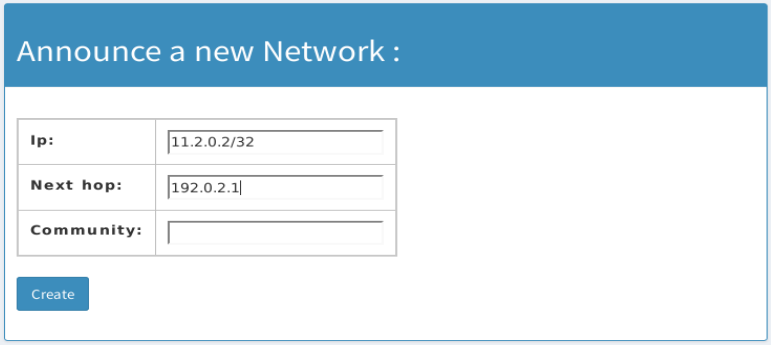
\includegraphics[width=\textwidth, height=0.45\textheight]{destination_based_target.png}
\end{frame}

\begin{frame}{Nos réalisations}{Redirection vers trou noir par la destination}
    {\large \centerline{État après la redirection}}
    \begin{minipage}{0.49\textwidth}
        \begin{figure}[H]
            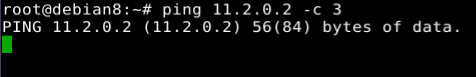
\includegraphics[width=\textwidth]{client_after_ban_destination_based_v2.png}
            \caption*{Client}
        \end{figure}
    \end{minipage}
    \hfill
    \begin{minipage}{0.49\textwidth}
        \begin{figure}[H]
            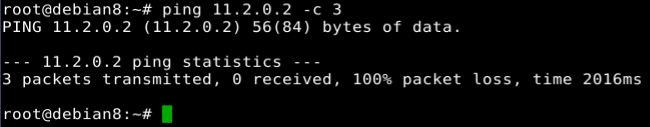
\includegraphics[width=\textwidth]{attacker_after_ban_destination_based_v2.png}
            \caption*{Attaquant}
        \end{figure}
    \end{minipage}

    \begin{alertblock}{Attention}
        Le déni de service est effectif
    \end{alertblock}
\end{frame}

\begin{frame}{Nos réalisations}{Redirection vers trou noir par la source}
    \begin{minipage}{0.5\textwidth}
        {\large Redirection par la source}
        \begin{figure}
            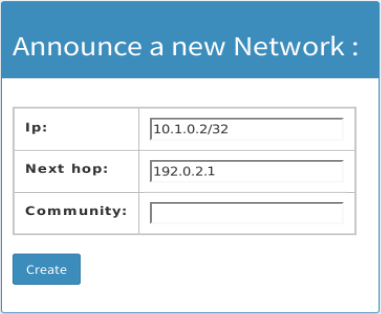
\includegraphics[width=\textwidth, height=0.7\textheight]{source_based_v2.png}
        \end{figure}
    \end{minipage}
    \hfill
    \begin{minipage}{0.38\textwidth}
        {\large État après la redirection}
        \begin{figure}[H]
            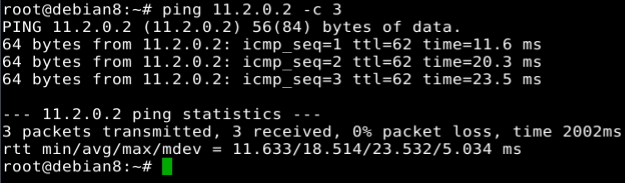
\includegraphics[width=\textwidth]{client_after_source_based_v2.png}
            \caption*{Client}
        \end{figure}

        \begin{figure}[H]
            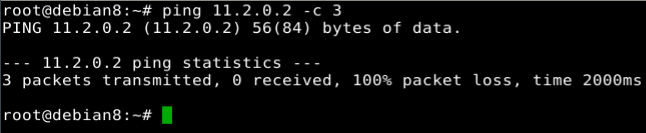
\includegraphics[width=\textwidth]{attacker_just_after_source_based_v2.png}
            \caption*{Attaquant juste après l'annonce}
        \end{figure}

        \begin{alertblock}{Mais}
            Après 60 secondes, la synchronisation est effective
        \end{alertblock}
    \end{minipage}
\end{frame}

\begin{frame}{Nos réalisations}{Redirection vers trou noir par la source}

    {\large {\color{cyan}L'attaquant peut recontacter la target via eth1}}
    \begin{figure}[H]
        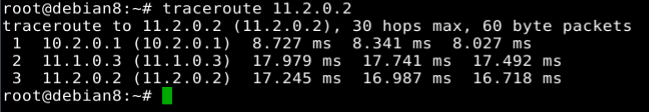
\includegraphics[width=\textwidth]{attacker_traceroute_30seconds_after_source_based_v2.png}
        \caption*{Traceroute sur l'attaquant}
    \end{figure}

    {\large {\color{red}Solution rediriger les deux interfaces vers le trou noir}}
    \begin{figure}[H]
        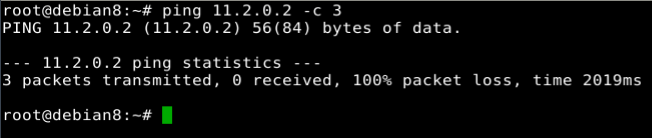
\includegraphics[width=\textwidth]{attacker_after_both_source_destination_v2.png}
        \caption*{Traceroute sur l'attaquant}
    \end{figure}

\end{frame}